
\tikzset{every picture/.style={line width=0.75pt}} %set default line width to 0.75pt        

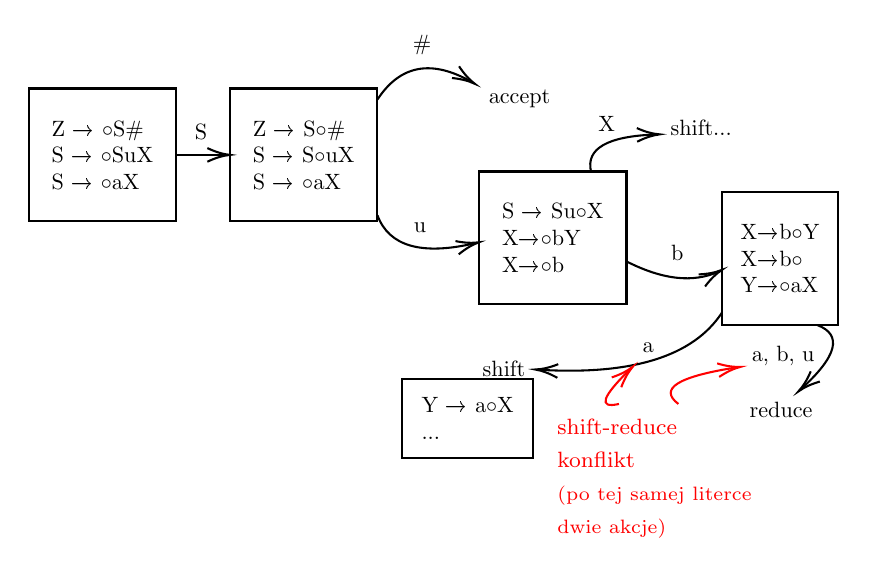
\begin{tikzpicture}[x=0.75pt,y=0.75pt,yscale=-1,xscale=1]

%uncomment if require: \path (0,300); %set diagram left start at 0, and has height of 300


% Text Node
\draw    (8,28) -- (79,28) -- (79,92) -- (8,92) -- cycle  ;
\draw (43.5,60) node [scale=0.8] [align=left] {Z → $\displaystyle \circ $S\#\\S → $\displaystyle \circ $SuX\\S → $\displaystyle \circ $aX};
% Text Node
\draw    (105,28) -- (176,28) -- (176,92) -- (105,92) -- cycle  ;
\draw (140.5,60) node [scale=0.8] [align=left] {Z → S$\displaystyle \circ $\#\\S → S$\displaystyle \circ $uX\\S → $\displaystyle \circ $aX};
% Text Node
\draw    (225,68) -- (296,68) -- (296,132) -- (225,132) -- cycle  ;
\draw (260.5,100) node [scale=0.8] [align=left] {S → Su$\displaystyle \circ $X\\X→$\displaystyle \circ $bY\\X→$\displaystyle \circ $b};
% Text Node
\draw    (342,78) -- (398,78) -- (398,142) -- (342,142) -- cycle  ;
\draw (370,110) node [scale=0.8] [align=left] {X→b$\displaystyle \circ $Y\\X→b$\displaystyle \circ $\\Y→$\displaystyle \circ $aX};
% Text Node
\draw (244.5,33) node [scale=0.8] [align=left] {accept};
% Text Node
\draw (237,163) node [scale=0.8] [align=left] {shift};
% Text Node
\draw (91,49) node [scale=0.8] [align=left] {S};
% Text Node
\draw (197.5,7) node [scale=0.8] [align=left] {\#};
% Text Node
\draw (320.5,107) node [scale=0.8] [align=left] {b};
% Text Node
\draw (306.5,153) node [scale=0.8] [align=left] {a};
% Text Node
\draw (370.5,183) node [scale=0.8] [align=left] {reduce};
% Text Node
\draw (371.5,157) node [scale=0.8] [align=left] {a, b, u};
% Text Node
\draw    (188,168) -- (251,168) -- (251,206) -- (188,206) -- cycle  ;
\draw (219.5,187) node [scale=0.8] [align=left] {Y → a$\displaystyle \circ $X\\...};
% Text Node
\draw (196.5,95) node [scale=0.8] [align=left] {u};
% Text Node
\draw (332,47) node [scale=0.8] [align=left] {shift...};
% Text Node
\draw (286.5,45) node [scale=0.8] [align=left] {X};
% Text Node
\draw (309.5,216) node  [align=left] {{\footnotesize \textcolor[rgb]{1,0,0}{shift-reduce}}\\{\footnotesize \textcolor[rgb]{1,0,0}{konflikt}}\\\textcolor[rgb]{1,0,0}{{\scriptsize (po tej samej literce}}\\\textcolor[rgb]{1,0,0}{{\scriptsize dwie akcje)}}};
% Connection
\draw    (79,60) -- (103,60) ;
\draw [shift={(105,60)}, rotate = 180] [color={rgb, 255:red, 0; green, 0; blue, 0 }  ][line width=0.75]    (10.93,-3.29) .. controls (6.95,-1.4) and (3.31,-0.3) .. (0,0) .. controls (3.31,0.3) and (6.95,1.4) .. (10.93,3.29)   ;

% Connection
\draw    (176,89.04) .. controls (181.56,104.13) and (197.36,108.61) .. (223.39,102.47) ;
\draw [shift={(225,102.08)}, rotate = 526.04] [color={rgb, 255:red, 0; green, 0; blue, 0 }  ][line width=0.75]    (10.93,-3.29) .. controls (6.95,-1.4) and (3.31,-0.3) .. (0,0) .. controls (3.31,0.3) and (6.95,1.4) .. (10.93,3.29)   ;

% Connection
\draw    (296,111.32) .. controls (313.43,120.16) and (328.19,121.8) .. (340.31,116.23) ;
\draw [shift={(342,115.39)}, rotate = 512.21] [color={rgb, 255:red, 0; green, 0; blue, 0 }  ][line width=0.75]    (10.93,-3.29) .. controls (6.95,-1.4) and (3.31,-0.3) .. (0,0) .. controls (3.31,0.3) and (6.95,1.4) .. (10.93,3.29)   ;

% Connection
\draw    (176,33.36) .. controls (186.96,16.6) and (202.13,13.79) .. (221.5,24.91) ;
\draw [shift={(223,25.79)}, rotate = 211.15] [color={rgb, 255:red, 0; green, 0; blue, 0 }  ][line width=0.75]    (10.93,-3.29) .. controls (6.95,-1.4) and (3.31,-0.3) .. (0,0) .. controls (3.31,0.3) and (6.95,1.4) .. (10.93,3.29)   ;

% Connection
\draw    (342,136.01) .. controls (328.14,157.13) and (298.6,166.28) .. (253.38,163.48) ;
\draw [shift={(252,163.39)}, rotate = 363.82] [color={rgb, 255:red, 0; green, 0; blue, 0 }  ][line width=0.75]    (10.93,-3.29) .. controls (6.95,-1.4) and (3.31,-0.3) .. (0,0) .. controls (3.31,0.3) and (6.95,1.4) .. (10.93,3.29)   ;

% Connection
\draw    (388,142) .. controls (400.19,146.69) and (397.57,156.94) .. (380.16,172.77) ;
\draw [shift={(378.79,174)}, rotate = 318.44] [color={rgb, 255:red, 0; green, 0; blue, 0 }  ][line width=0.75]    (10.93,-3.29) .. controls (6.95,-1.4) and (3.31,-0.3) .. (0,0) .. controls (3.31,0.3) and (6.95,1.4) .. (10.93,3.29)   ;

% Connection
\draw    (278.9,68) .. controls (276.37,56.95) and (286.79,51) .. (310.18,50.17) ;
\draw [shift={(312,50.11)}, rotate = 538.64] [color={rgb, 255:red, 0; green, 0; blue, 0 }  ][line width=0.75]    (10.93,-3.29) .. controls (6.95,-1.4) and (3.31,-0.3) .. (0,0) .. controls (3.31,0.3) and (6.95,1.4) .. (10.93,3.29)   ;

% Connection
\draw [color={rgb, 255:red, 255; green, 0; blue, 0 }  ,draw opacity=1 ]   (321,180) .. controls (311.33,172.63) and (320.74,166.76) .. (349.23,162.37) ;
\draw [shift={(351,162.11)}, rotate = 531.5899999999999] [color={rgb, 255:red, 255; green, 0; blue, 0 }  ,draw opacity=1 ][line width=0.75]    (10.93,-3.29) .. controls (6.95,-1.4) and (3.31,-0.3) .. (0,0) .. controls (3.31,0.3) and (6.95,1.4) .. (10.93,3.29)   ;

% Connection
\draw [color={rgb, 255:red, 255; green, 0; blue, 0 }  ,draw opacity=1 ]   (292.38,180) .. controls (282.19,182.3) and (283.99,176.72) .. (297.77,163.27) ;
\draw [shift={(299.09,162)}, rotate = 496.19] [color={rgb, 255:red, 255; green, 0; blue, 0 }  ,draw opacity=1 ][line width=0.75]    (10.93,-3.29) .. controls (6.95,-1.4) and (3.31,-0.3) .. (0,0) .. controls (3.31,0.3) and (6.95,1.4) .. (10.93,3.29)   ;


\end{tikzpicture}
